\section{Injection of new physics models}
\label{sec:NewPhysics}
In looking at possible signal models, we have chosen three that we
believe will be representative of many models.  These are a
technicolor $\rho_T \ra \Wo\pi_T$~\cite{Eichten:2011sh}, a leptophobic $\Zo^\prime
\ra jj~$\cite{Buckley:2011vc}, and a Standard Model Higgs produced in
association with a \Wo\ or \Zo.  This gives us a scalar resonance, a
pseudo-scalar resonance, and a vector resonance, as well as one that
additionally should have a peak in the four body mass. The cross-sections
and efficiency numbers are given in Table~\ref{tab:signals}.
%%%%%%%%%%%
%%%%%%%%%%%
 The dijet mass spectrum for a Higgs and a leptophobic $\Zo^{\prime}$
are shown in Fig.~\ref{fig:NewPhysicsMjj}. The dijet and W$jj$ spectra
for the technicolor model are shown in Fig.~\ref{fig:tc}.
%%%%%%%
\begin{figure}[h!] {\centering
\unitlength=0.33\linewidth
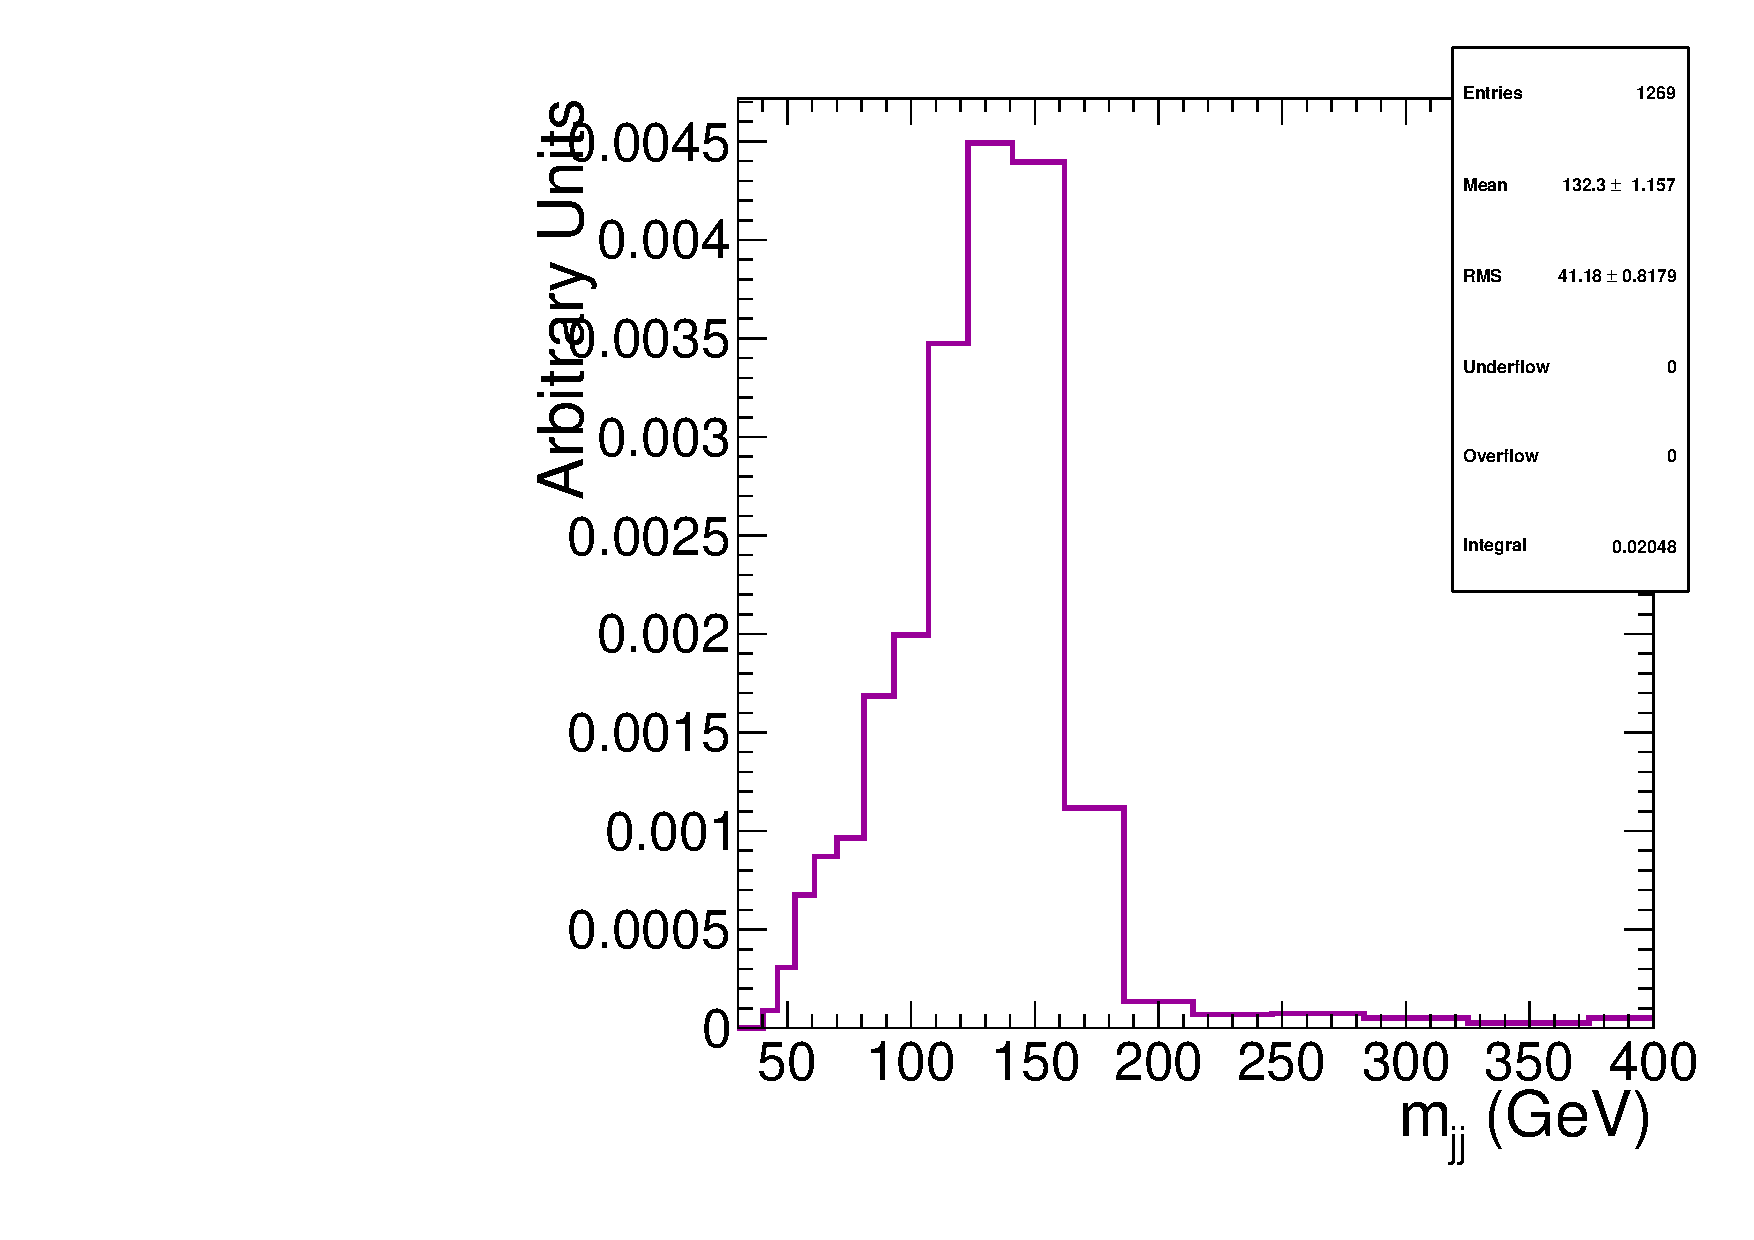
\includegraphics[width=0.48\textwidth]{figs/WHZH_mjj}
\put(-0.80,0.0){(a)} 
\unitlength=0.33\linewidth
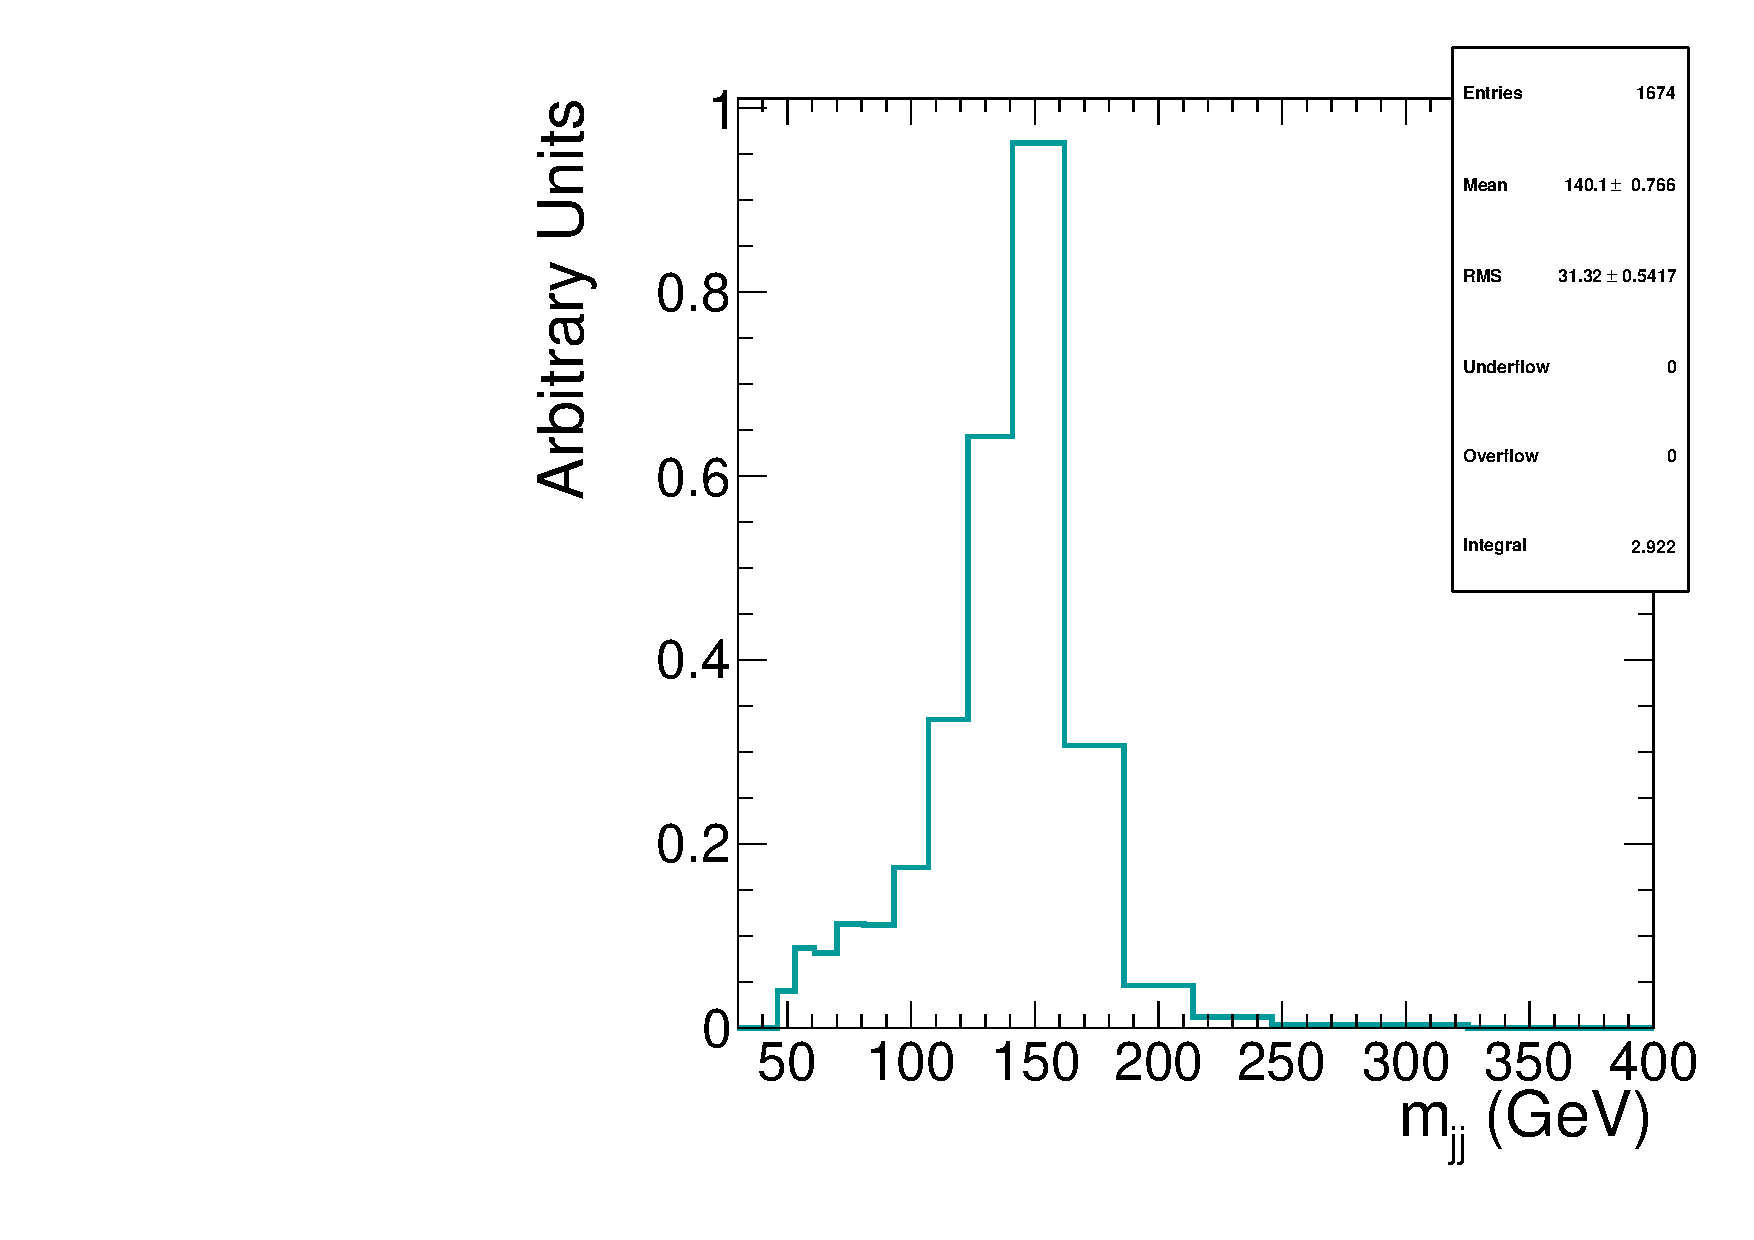
\includegraphics[width=0.48\textwidth]{figs/Zprime_mjj}
\put(-0.80,0.0){(b)} 
\caption{Dijet mass spectrum for New Physics events: 
(a) $\Wo\mathrm{H}$/$\Zo\mathrm{H}$ and 
(b) leptophobic $\Zo^\prime$.
} 
\label{fig:NewPhysicsMjj}}
\end{figure}
%%%%%%%
%%%%%%%%%%%
%%%%%%%%%%%
\begin{figure}[bthp]
\begin{center}
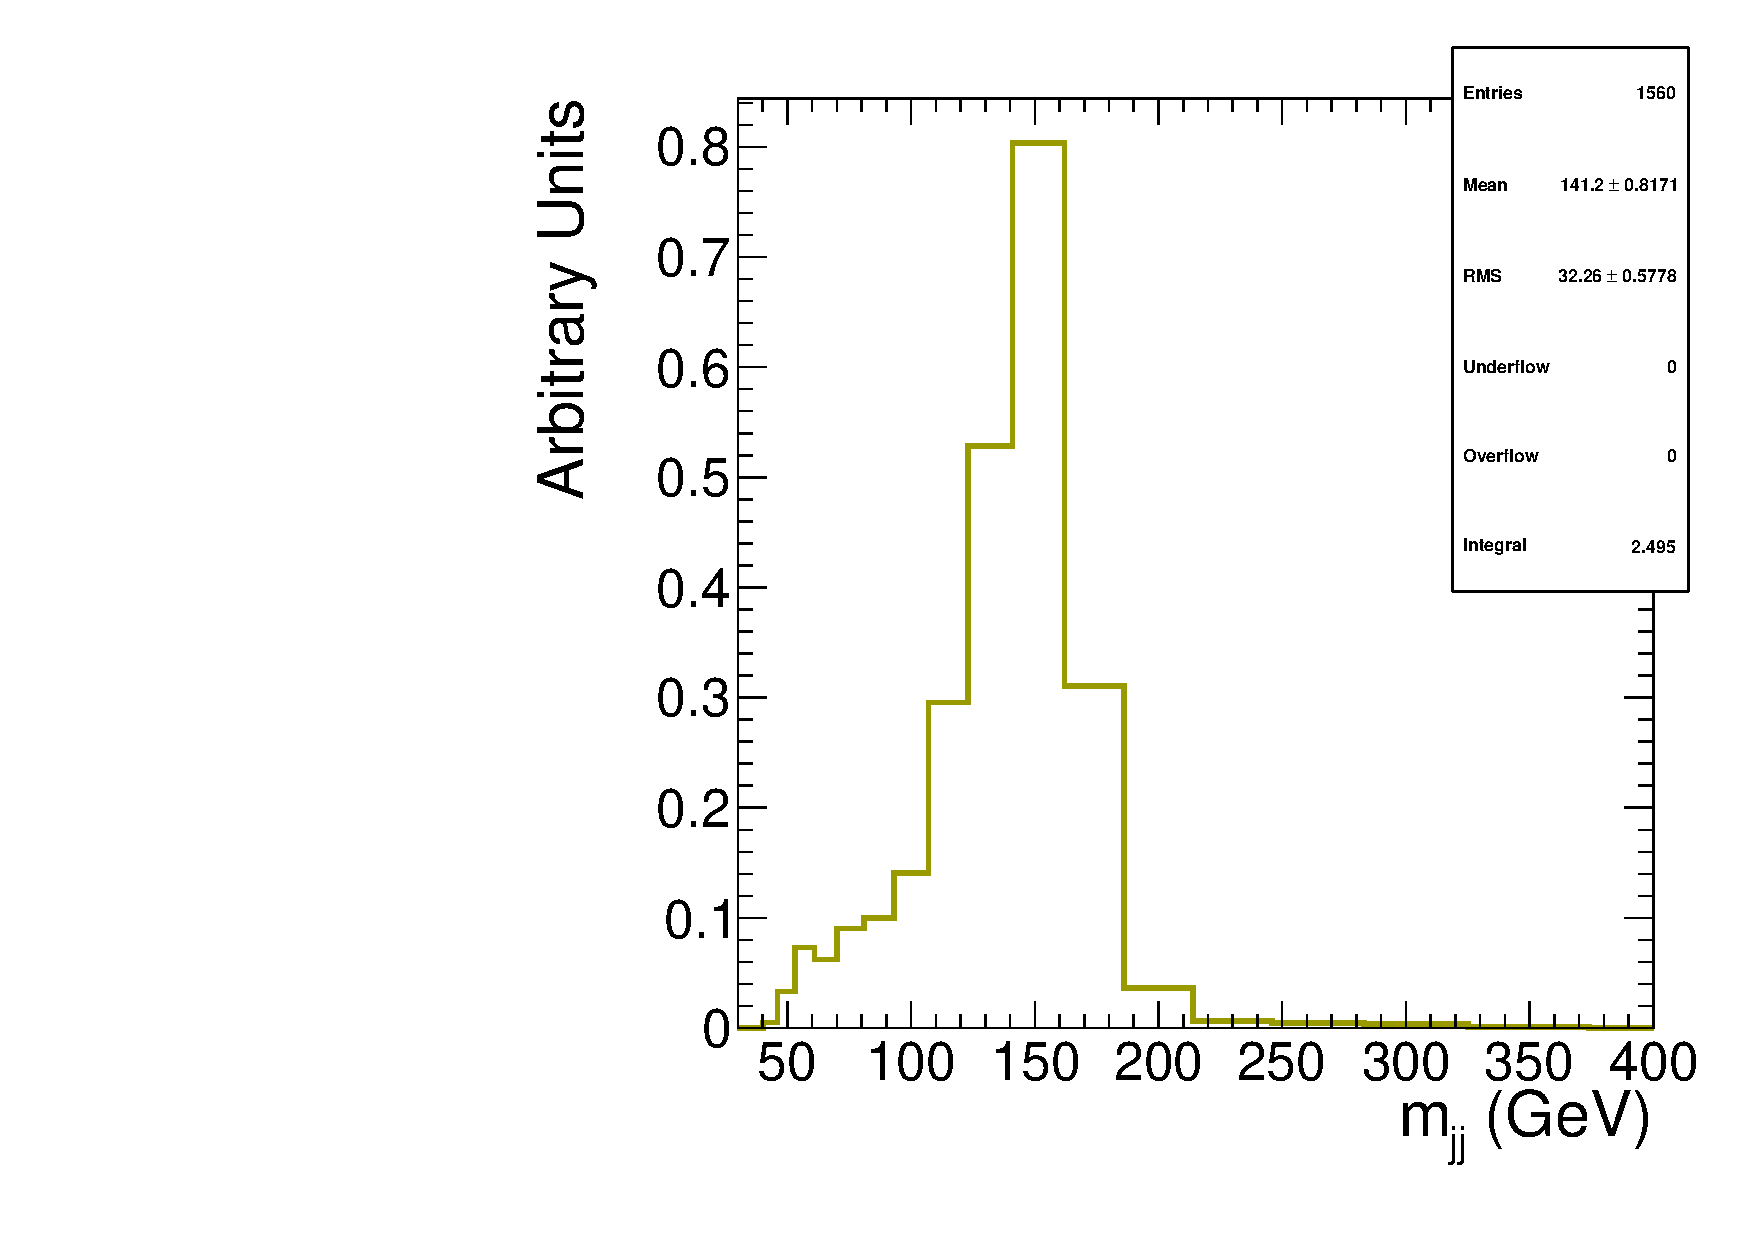
\includegraphics[width=0.475\columnwidth]{figs/Technicolor_mjj}
%\makebox[0.475\columnwidth][c]{plot coming soon}
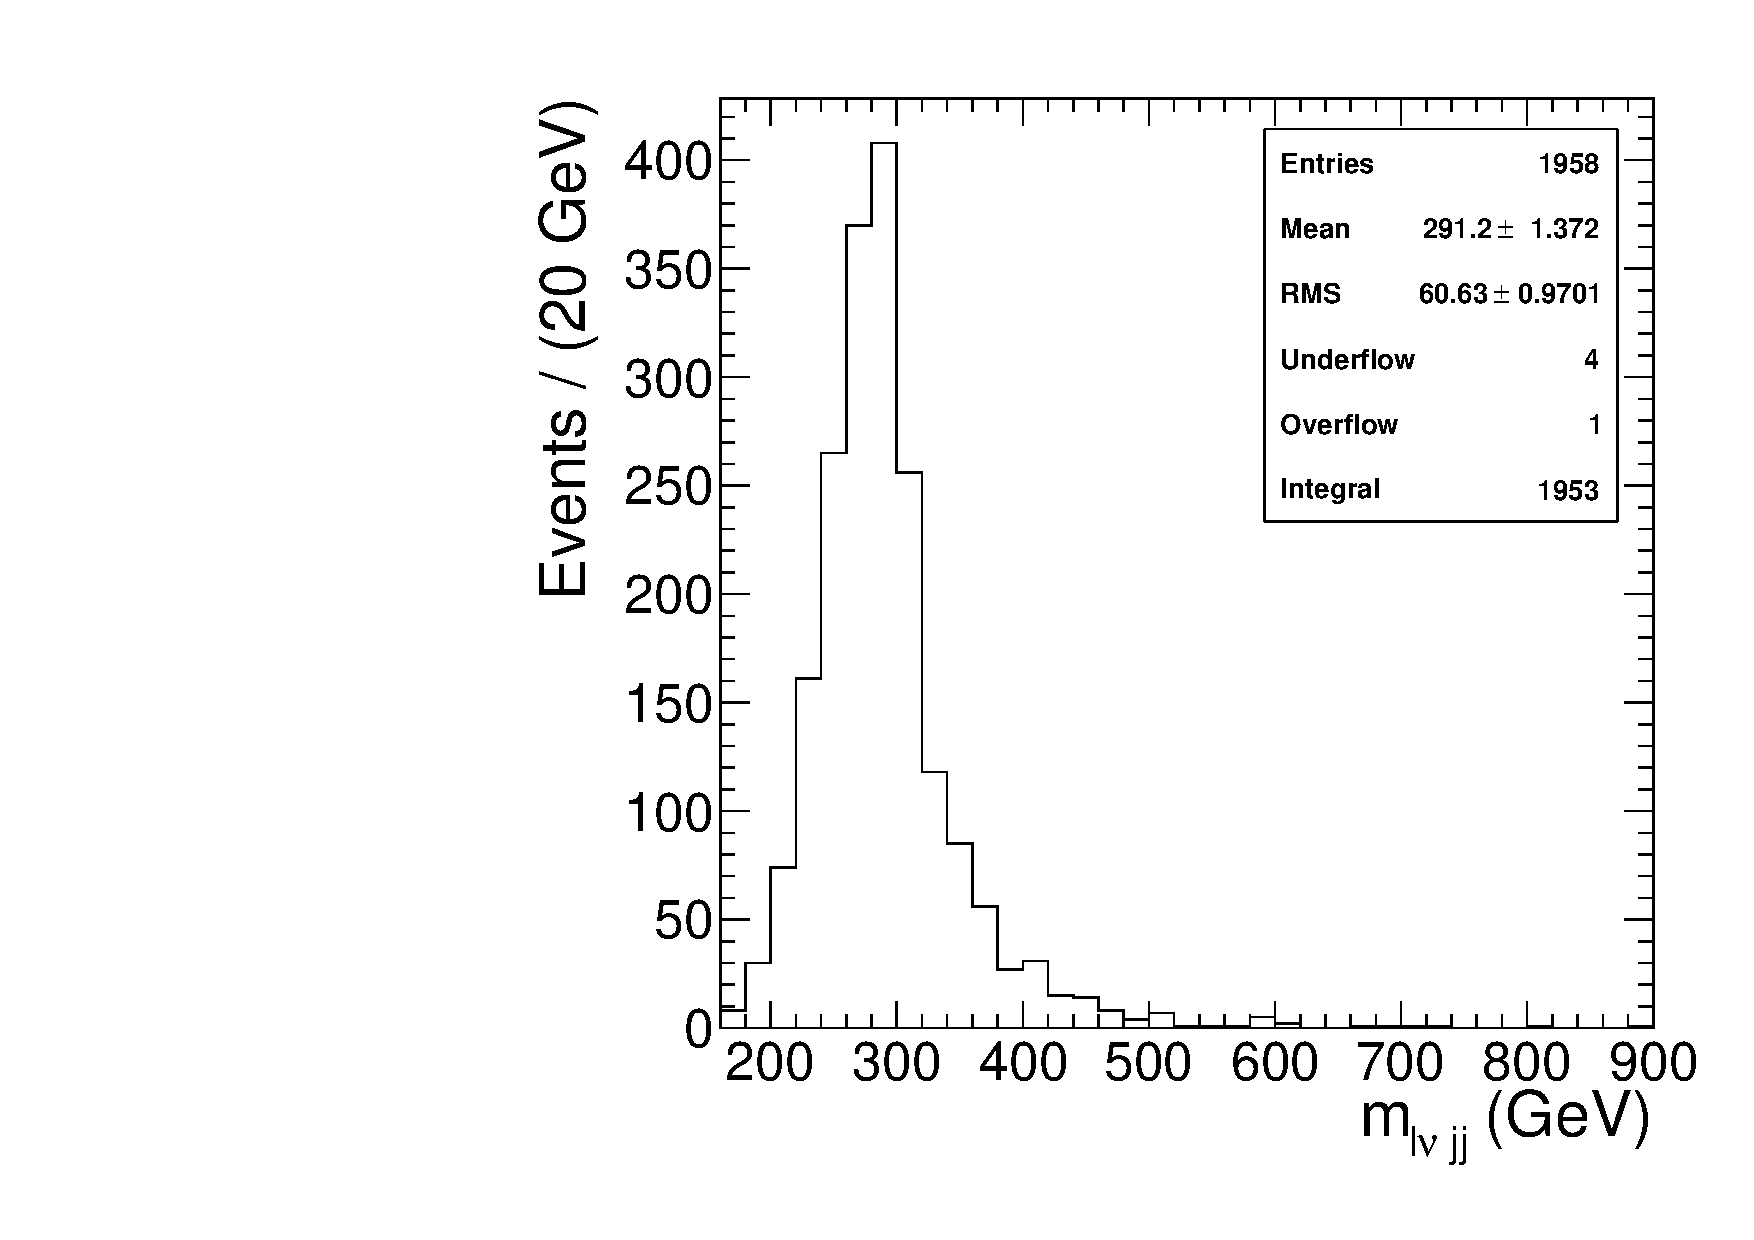
\includegraphics[width=0.475\columnwidth]{figs/Technicolor_mWjj}
\end{center}
\caption{\label{fig:tc}Dijet mass distribution (left) and $\Wo jj$
  mass distribution (right) for a Technicolor model.}
\end{figure}
%%%%%%%%%%%
%%%%%%%%%%%%%%%%%%%%%%%
\subsection{WH/ZH}
These events were generated using Pythia using the Z2 tune and
standard pileup.  The details of the Pythia configuration are
\begin{verbatim}
  MSEL=0
  24:ALLOFF
  24:ONIFANY 13 11
  23:ALLOFF
  23:ONIFANY 11 13
  MSUB(24)=1
  MSUB(26)=1
  PMAS(25,1)=150.0
\end{verbatim}
Using this configuration, we generated 50k events with standard CMSSW
tools.
%%%%%%%%%%%%%%%%%%%%%%%
\subsection{\texorpdfstring{$\Zo^\prime$}{Z-prime}}
For a leptophobic $\Zo^\prime$, 50k events were generated via MadGraph
in LHE format and provided to us~\cite{BuckleyMC},
\cite{Buckley:2011vc}.  These events were processed using the standard
CMSSW tools.
%%%%%%%%%%%%%%%%%%%%%%%
\subsection{Technicolor}
For the technicolor model we received a Pythia configuration~\cite{AMartinMC},~\cite{Eichten:2011sh},
shown below.
\begin{verbatim}
  MSEL=0
  MSUB(362)=1
  MSUB(368)=1
  MSUB(371)=1
  MSUB(376)=1
  MSUB(366)=0
  MSUB(372)=0
  MSUB(375)=0
  PMAS(329,1)=160.0d0
  PMAS(330,1)=160.0d0
  PMAS(333,1)=290.0d0
  PMAS(334,1)=290.0d0
  PMAS(335,1)=290.0d0
  PMAS(368,1)=320.0d0
  RTCM(12)=290.0d0
  RTCM(13)=290.0d0
  RTCM(48)=290.0d0
  RTCM(49)=290.0d0
  RTCM(50)=1000.0d0
  RTCM(51)=1000.0d0
  MDME(174,1)=0
  MDME(175,1)=0
  MDME(176,1)=0
  MDME(177,1)=0
  MDME(178,1)=0
  MDME(179,1)=0
  MDME(182,1)=0
  MDME(184,1)=0
  MDME(186,1)=0
  MDME(190,1)=0
  MDME(191,1)=0
  MDME(192,1)=0
  MDME(194,1)=0
  MDME(195,1)=0
  MDME(196,1)=0
  MDME(198,1)=0
  MDME(199,1)=0
  MDME(200,1)=0
  MDME(208,1)=0
  24:ALLOFF
  24:ONIFANY 11 13
\end{verbatim}
Using Pythia and the standard CMSSW tools we generated 50k events.
%%%%%%%%%%%%%%%%%%%%%%%%%%%%
%%%%%%%%%%%%%%%%%%%%%%%%%%%%
%%%%%%%%%%%%%%%%%%%%%%%%%%%%
\subsection{Attempt to understand jet flavor expectation in these models}
The technicolor model provided by "ELM" has
arbitrarily selected coupling constants for the mixing
between techni-$\pi^0$ and techni-$\pi^{0'}$.
%%
%% ``Thanks to Steve for pointing this out to us.''
%%
We therefore list here the branching ratios of the techni-color
particles used in this model.
\par
The techni-$\pi^+$  decays to heavy flavor with
BR=81\%  but cannot decay to gluons.
The techni-$\pi^0$  decays to heavy flavor
with BR=87\%  and again cannot decay to gluons.
The techni-$\pi^{0'}$ decays to heavy flavor
with BR=49\% and decays to a gluon pair with
BR=44\%. The mixing is such that the techni-$\pi^{0'}$
component is small.

\par
This explains the loss of efficiency
by a factor of 2/3 when applying an anti-$b$-tag and another
big loss when applying a quark-gluon likelihood cut.

The detailed tables of the branching ratio for
each technicolor particle, generated by Pythia, are printed below:

\begin{verbatim}
  3000111    329    pi_tc0                              0
         3996    1   32    0.025601    s            sbar
         3997    1   32    0.044880    c            cbar
         3998    1   32    0.825258    b            bbar
         3999    1   32    0.000000    t             tbar
         4000    1    0    0.000000    e-            e+
         4001    1    0    0.000367    mu-        mu+
         4002    1    0    0.103894    tau-        tau+
         4003    1   32    0.000000    g             g


  3000211    330    pi_tc+          pi_tc-              3
         4004    1   32    0.019814    c            dbar
         4005    1   32    0.023328    c            sbar
         4006    1   32    0.361831    u            bbar
         4007    1   32    0.549403    c            bbar
         4008    1   32    0.000000    W+         b bbar
         4009    1    0    0.000000    e+           nu_e
         4010    1    0    0.000161    mu+        nu_mu
         4011    1    0    0.045463    tau+        nu_tau


  3000221    331    pi'_tc0                             0
         4012    1   32    0.013695    s              sbar
         4013    1   32    0.025421    c              cbar
         4014    1   32    0.466595    b             bbar
         4015    1   32    0.000000    t               tbar
         4016    1    0    0.000000    e-              e+
         4017    1    0    0.000196    mu-          mu+
         4018    1    0    0.055451    tau-          tau+
         4019    1   32    0.438642    g               g

\end{verbatim}

The Z' signal doesn't suffer from heavy flavor or gluon contamination
because it decays most frequently to light flavor qqbar pairs (Matt Buckley/
Dan Hooper model has $pp\to WZ' \to Wjj$). The WH sample has a
significant fraction of heavy flavor because the Higgs boson couples
mostly to $b\bar{b}$. Therefore, we do not apply an anti-$b$-tag or
quark-gluon likelihood cut, because such a cut would discriminate
against technicolor- and WH-type signals.
